\documentclass[a4paper]{article}

\usepackage[french]{babel}
\usepackage[T1]{fontenc}
\usepackage[utf8]{inputenc}
\usepackage{amsmath}
\usepackage{graphicx}
\usepackage{tikz}
\usepackage{adjustbox}
\usepackage{lmodern}
\usepackage[left=3cm, right=3cm, bottom=4cm, top=4cm]{geometry}
\usepackage{array}
\usepackage{pdfpages}

\usepackage[gen]{eurosym}
\DeclareUnicodeCharacter{20AC}{\euro{}}

\usepackage{hyperref}
\usepackage{xcolor}
\hypersetup{
    colorlinks,
    linkcolor={blue!50!black},
    citecolor={blue!50!black},
    urlcolor={blue!80!black}
}


\title{\textbf{Rapport de projet d'acquisition de connaissances}\\Étude d’un moteur de recherche existant et évaluation comparative}

\author
{
	Pierre-Marie {\sc Airiau}\\
    Hyuk-Chan {\sc Kwon}\\
    Maud {\sc Leray}\\
    Thibaut {\sc Rapin}\\
    Maxime {\sc Thebault}
}

\date{\today}

\newcommand{\pagevierge}[0]{\newpage\thispagestyle{empty}\null\newpage}

\newcommand{\annexe}[1]{%
	\clearpage
	\newpage
    \vspace*{-4cm}
	\refstepcounter{section}%
	\phantomsection%
	%\addcontentsline{toc}{section}{\appendixname~{\thesection}: #1}%
	\section*{\appendixname~{\thesection}: #1}
    }


\begin{document}
	\maketitle
	\thispagestyle{empty}
	\begin{tikzpicture}[remember picture, overlay]
   	 \node [anchor=south west, inner sep=10pt, outer sep=80pt]  at (current page.south west)
   	  {
\includegraphics[width=4cm]{figure/logo_insa.png}};
     \node [anchor=south east, inner sep=20pt, outer sep=80pt]  at (current page.south east)
	  {
\includegraphics[width=4cm]{figure/logo_lucene.png}};
	\end{tikzpicture}
    % Ouh c'est sale.
    \hypersetup{pageanchor=false}
    %
\includepdf[pages=1]{figure/couv.pdf}
    \hypersetup{pageanchor=true}
    
    \newpage
    \thispagestyle{empty}
    \mbox{}
    
    \newpage
    % A decommenter pour la release
    \setcounter{tocdepth}{2}
    \tableofcontents
    \setlength{\parskip}{10pt}
    
    \newpage
    \thispagestyle{empty}
    \mbox{}
    
    \newpage
    \section{Introduction}

Ce document rend compte d’un travail effectué en 4^{e} année du département informatique de l’INSA de Rennes dans le domaine de l’acquisition de connaissances, et plus spécifiquement dans la recherche d’informations (information retrieval).

Nous avons choisi d’étudier le fonctionnement d’un moteur de recherche relativement répandu et d’en faire une étude comparative. Il s’agit d’évaluer différentes configurations de ce moteur de recherche sur une collection de documents fournies par l’université de Glasgow (collection CISI) suivant différents critères.

Dans un premier temps, nous présentons Lucene, le moteur de recherche testé. Après avoir exposé des généralités sur le logiciel, nous donnons un bref aperçu de son fonctionnement, pour enfin nous concentrer sur les aspects pouvant être configurés. Nous abordons ainsi la notion d’analyseur, de termes et de filtres.

Dans un deuxième temps, nous décrivons la méthodologie utilisée pour l’étude comparative. On spécifie le processus de test et nous détaillons les critères utilisés pour l’évaluation.

S’en suit une présentation du programme réalisé. Il est chargé d’exécuter les différents tests et d’en retirer les critères évoqués précédemment. Nous évoquons dans cette partie les aspects les plus techniques de ce rapport, puisqu’il s’agit là de l’implémentation du banc de test tel qu’il aura été spécifié dans les parties précédentes.

Enfin, nous analysons les résultats des tests menés. Dans un premier temps, nous détaillons les configurations que nous avons choisi d’évaluer avant d’étudier dans un second temps les performances de chacune. Nous concluons cette partie avec une synthèse donnant les configurations optimales en fonction des critères retenus.


























\newpage
    \section{Lucene}

Dans cette première partie, nous abordons Lucene, le moteur de recherche que nous avons choisi d’évaluer. Après une présentation général du projet Lucene, nous donnons un aperçu de son fonctionnement pour ensuite entrer dans les détails des composants pouvant être configurées.

\subsection{Généralités}

Lucene est une bibliothèque libre codée en Java proposant des fonctionnalités avancées d’indexation et de recherche de documents. Elle a été créée en 1999 par Doug Cutting, qui a par ailleurs créé Hadoop, très utilisé dans le domaine de la Big Data. Lucene devient en 2001 un projet Apache, lui conférant ainsi une certaine notoriété auprès du public.

Avant l’explosion d’Internet, la masse et la variété des documents présents sur la Toile étaient encore modestes : la méthode de recherche plébiscitée était la classification décimale de Dewey, dont s’inspire encore les bibliothèques. Avec cette méthode, il y a 3 niveaux de classification : les classes, les divisions et les sections. Les classes sont au nombre de 10. On retrouve par exemple la classe “religion”, la classe “langues”, la classe “sciences sociales”, etc. Les divisions sont l’équivalent des sous-catégories, elles sont au nombre de 100. Enfin, les sections permettent une nouvelle fois de raffiner la catégorie des documents classés, elles sont au nombre de 1000.

Bien que cette classification soit intuitive, elle pose de multiples problèmes : elle est assez statique et doit être modifiée quand de nouveaux types de documents apparaissent, elle ne permet pas les recherches ciblées sur des mots-clés et les recherches ne sont pas efficaces dû au trop grand nombre d’indirections. Enfin, l’explosion du nombre de documents disponibles sur Internet a montré les limites de cette classification : même avec 1000 sections différentes, le nombre de documents disponibles dans chacune des catégories est devenu trop important.

Pour explorer le web, la méthode de référence est devenue la recherche par mots-clés, elle est aujourd’hui utilisée par la très grande majorité des moteurs de recherche grand public. Pour permettre une recherche rapide et efficace parmi la masse importante de documents, une nouvelle approche était nécessaire : c’est celle que fournit Lucene.

La bibliothèque est aujourd’hui utilisée par des sites web comme Wikipedia, Akamai ou SourceForge ; mais elle est aussi utilisée par des applications telles que Eclipse, JIRA, Nutch ou Solr (ces deux dernières applications étant elles-mêmes des outils de plus haut niveau que Lucene facilitant la mise en place d’un moteur de recherche). Grâce à ses très bonnes performances et sa fiabilité, elle est au cœur de nombreux projets traitant de la récupération d’informations.

\subsection{Fonctionnement général}

Pour s’affranchir de potentiels problèmes de format (PDF, HTML, Word, etc.), Lucene a créé sa propre abstraction. Ainsi, l’objet manipulé par la bibliothèque logicielle est le document, qui est composé d’un ou plusieurs champs qui contiennent du texte.
L’utilisation de Lucene est décomposée en deux grandes parties : la première étape consiste en l’indexation des documents. C’est seulement après cette étape que l’on pourra interroger Lucene pour retrouver les documents correspondants à une requête de l’utilisateur.

\subsubsection{Indexation}

Pour cette première étape, il faut avant tout extraire le texte que l’on veut indexer d’un fichier HTML, PDF ou Word (cette tâche n’est pas assurée par Lucene et est à la charge du programmeur). Ensuite, il faut en créer un document. Par exemple, si l’on veut indexer une bibliothèque pour permettre à ses usagers de trouver un livre à partir de mots-clés de son résumé, on pourra utiliser la modélisation suivante pour les documents :

Le document représente un livre :
\begin{itemize}
  \item Un champ ISBN pour identifier un livre de manière unique
  \item Un champ titre
  \item Un champ auteur
  \item Un champ résumé
  \item Un champ rayon pour permettre de retrouver le livre dans la bibliothèque
\end{itemize}

~~\\
On remarque que tous les champs ne seront pas utiles à la recherche. Par exemple, l’usager d’une bibliothèque ne recherchera jamais un livre suivant sa position en rayon : s’il sait déjà où se trouve le livre, il saura déjà quel est le titre du livre, qui en est l’auteur, etc. En revanche, si l’utilisateur recherche un livre à partir de mots-clés du résumé, il peut être intéressant de lui indiquer où il se trouve dans la bibliothèque. Ainsi, le champ d’un document Lucene dispose de deux paramètres de configuration : “indexed” qui indique à Lucene via une valeur booléenne si le champ pourra faire l’objet d’une requête de l’usager (le paramètre sera par exemple à vrai pour le champ résumé, mais à faux pour le champ rayon), et “stored” qui indique si le champ sera affiché dans les résultats de la recherche. La performance de la recherche dépendra de ces paramètres. De manière logique, si l’on rend tous les champs cherchables (“indexed” à vrai), la recherche sera plus longue.

Une fois que le problème est modélisé sous forme de documents et de champs, et que ces derniers sont correctement configurés, nous pouvons procéder à l’indexation. Un index n’est rien d’autre qu’une forme condensée des documents en entrée permettant une recherche rapide et efficace. L’indexation permettra de créer et de mettre à jour l’index, tandis que l’interrogation se contentera de le consulter pour répondre à une requête de l’utilisateur.

\subsubsection{Interrogation}

L’étape d’interrogation peut devenir très complexe si l’on veut utiliser toutes les possibilités de recherche de Lucene, mais nous nous contentons dans cette partie de la version la plus basique.

Dans un premier temps, l’utilisateur entre sa requête : sur quel(s) terme(s) veut-il effectuer sa recherche ? Il revient ensuite au programmeur de faire l’intermédiaire entre l’utilisateur et Lucene : il faut configurer la recherche, en indiquant les champs dans lesquels on veut chercher les termes entrés par l’utilisateur (leurs paramètres de configuration “indexed” doivent obligatoirement être vrais), et les champs que l’on veut récupérer dans les résultats de la recherche (leurs paramètres de configuration “stored” doivent obligatoirement être vrais). Après consultation de l’index, Lucene nous renvoie des résultats et associe à chaque réponse un score, qui estime la pertinence du document retourné au vue de la requête de l’utilisateur.

Lucene propose de nombreuses autres possibilités de recherche : possibilité de trier les résultats sur un champ, possibilité de filtrer les résultats en fonction de la valeur d’un champ, possibilité de mise en surbrillance des termes d’un champ répondant à la requête de l’utilisateur, etc. Ces différentes fonctionnalités ne seront pas utiles à notre étude, et ne seront donc pas détaillées.

\subsubsection{Synthèse}

Une illustration synthétisant les concepts évoqués précédemment est disponible en annexe //TODO//, elle permet de distinguer clairement les responsabilités des différents acteurs (l’utilisateur, le programmeur et la bibliothèque logicielle Lucene) et indique le déroulement de l’indexation (à gauche) et de l'interrogation (à droite).

 \begin{figure}[h]
            \centering
            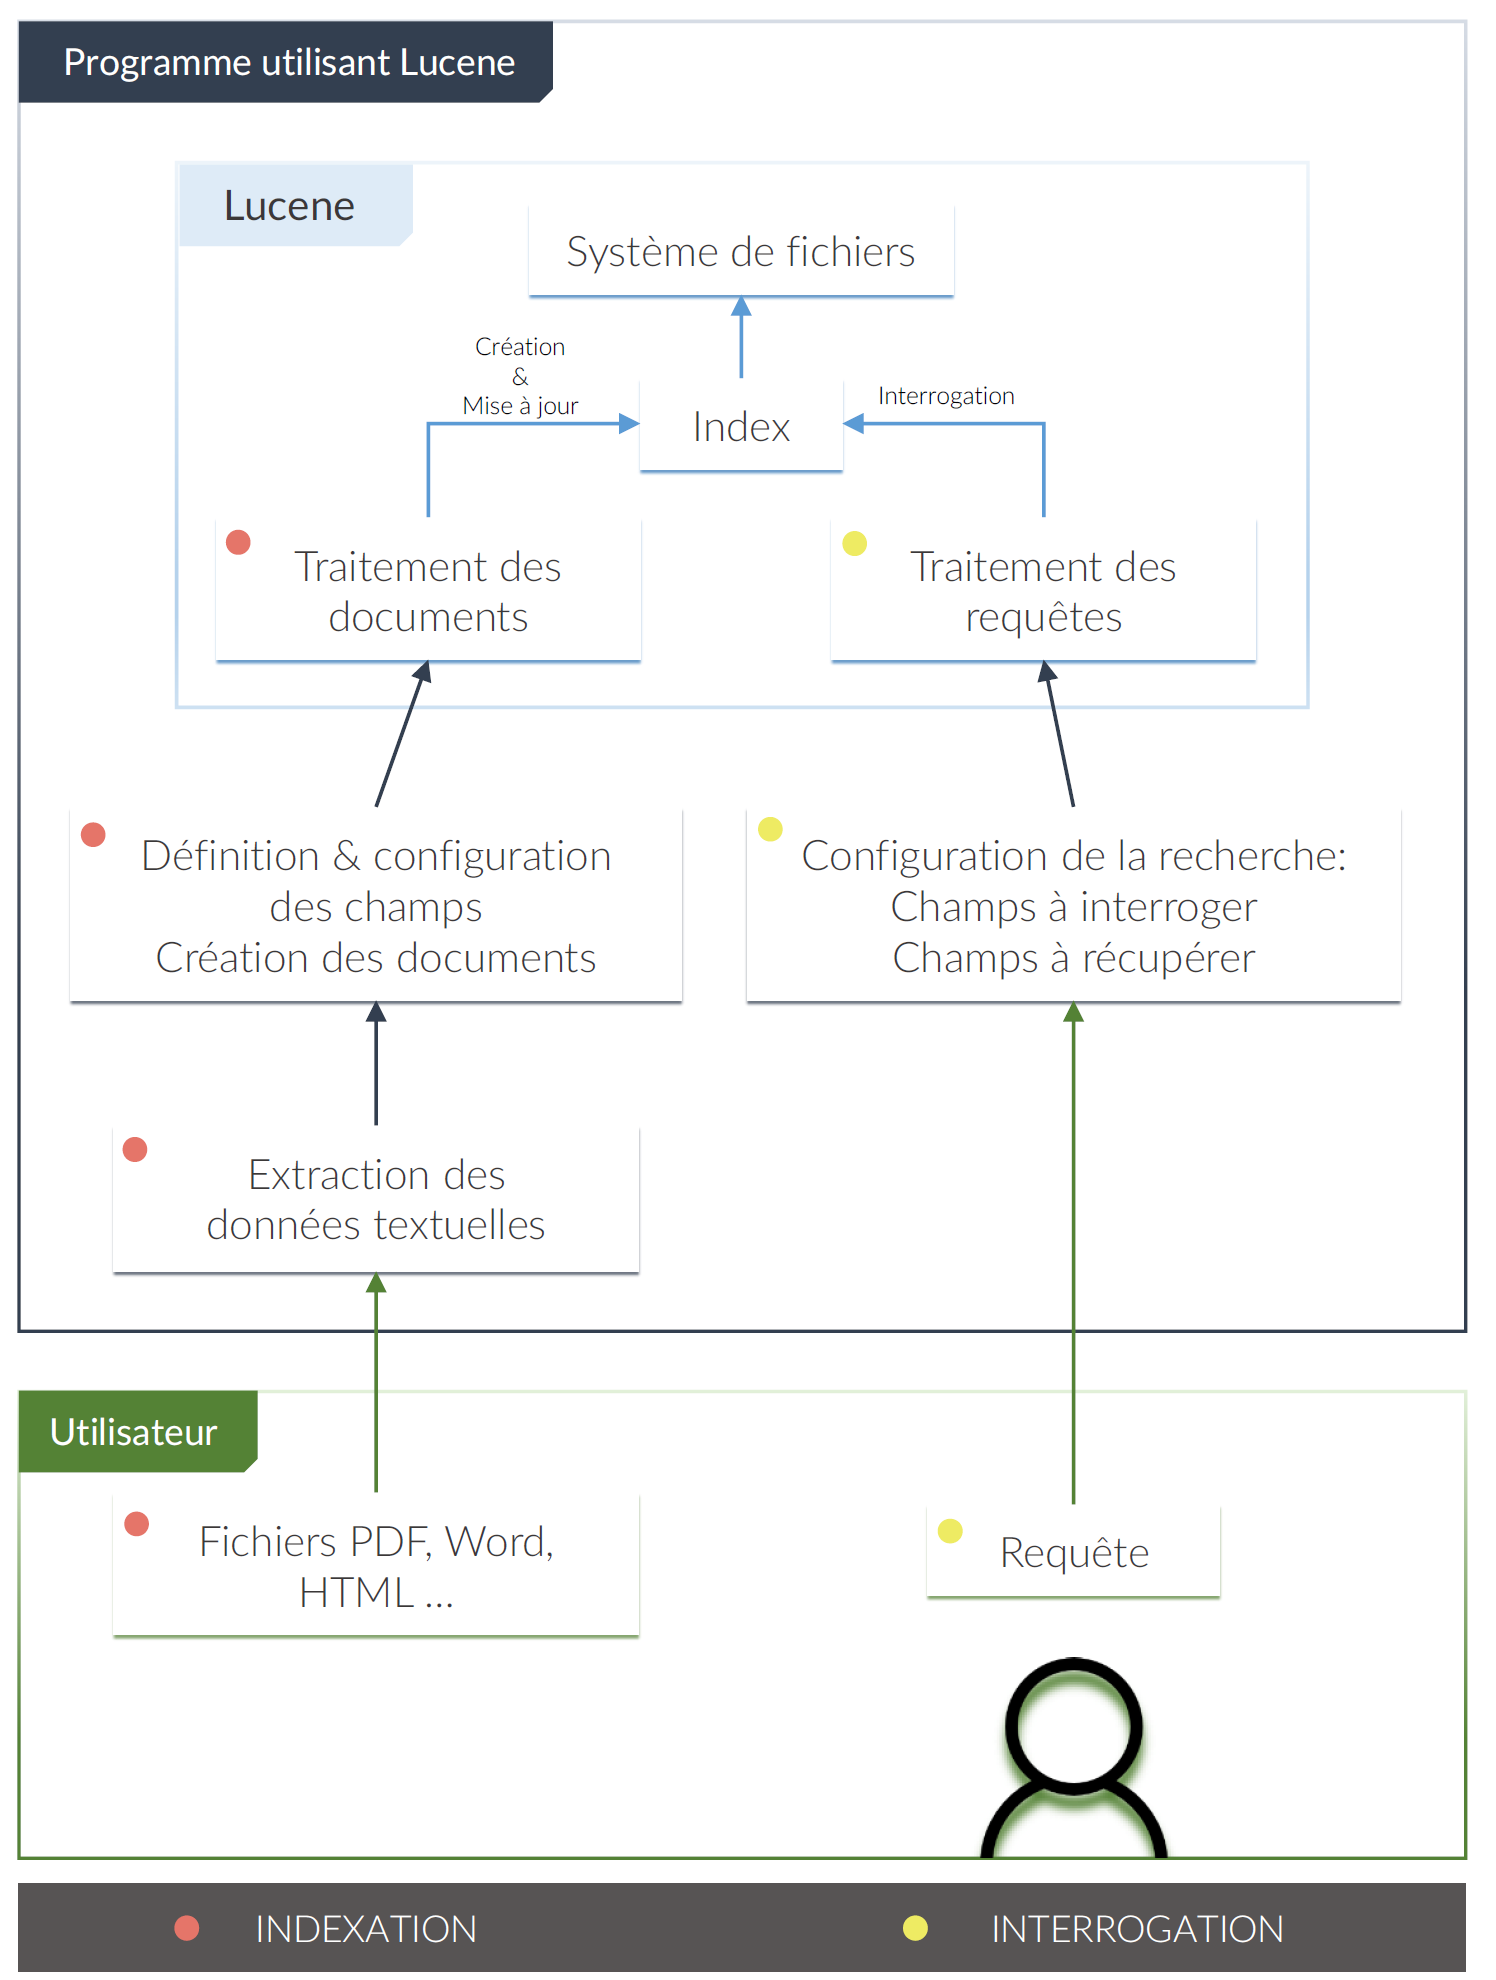
\includegraphics[width=12cm]{figure/fonctionnement.jpg}
            \caption{Fonctionnement programme}
            \label{fig:fonctionnement_prog}
 \end{figure}

\subsection{Analyseur}

Pour permettre une recherche efficace, le texte contenu dans les champs d’un document est transformé en une succession de termes. Cette étape est fondamentale pour assurer la pertinence des résultats : cela permettra par exemple de trouver une correspondance entre un verbe conjugué dans un document et un verbe à l’infinitif dans la requête d’un utilisateur. Il s’agira dans un premier temps de pouvoir distinguer les différents termes de la phrase, grâce au découpage en termes (tokenization en anglais). C’est sur ces termes qu’on appliquera des transformations, grâce au filtrage.

\subsubsection{Le découpage en termes}
\label{section:tokenizer}

Lucene met à disposition plusieurs tokenizers prédéfinis, dont le fonctionnement est synthétisé dans le tableau //TODO//. Pour illustrer leurs actions, la troisième colonne donne les différents termes produits pour le texte d’entrée “Voit-on J.M. demain ?”.
 
            \begin{table}[!htbp]
                \centering
                \begin{tabular}{|p{4.5cm}|p{4.5cm}|p{4.5cm}|}
                    \hline
                    \textbf{Nom} & \textbf{Fonctionnement} & \textbf{Termes produits}\\
                    \hline
                    KeywordTokenizer & Transforme l’ensemble du texte d’entrée en un unique terme & “Voit-on J.M. demain ?”\\
		\hline
                    WhitespaceTokenizer & Crée un nouveau terme à chaque espace blanc & “Voit-on” “J.M.” “demain”\\
		\hline
                    StandardTokenizer & Crée un nouveau terme à chaque séparateurs de mots couramment rencontrés dans les langages & “Voit” “on” “J.M.” “demain”\\
		\hline
                    LetterTokenizer & Crée un nouveau terme à chaque séparation de mots & “Voit” “on” “J” “M” “demain”\\
		\hline
                    LowerCaseTokenizer & Crée un nouveau terme à chaque séparation de mots en enlevant les majuscules & “voit” “on” “j” “m” “demain”\\
                    \hline

                \end{tabular}
                \caption{Découpage des termes}
                \label{tab:decoupage_termes}
            \end{table}

\subsubsection{Le filtrage des termes}
\label{section:filtres}

Après le découpage en termes vient l’étape de filtrage, pendant laquelle chacun des termes va être passé en revue. Ce traitement permettra soit de supprimer, soit de modifier, soit de créer de nouveaux termes. Le tableau //TODO// donne un aperçu des filtres les plus courants, et montre leurs effets sur des exemples :

\begin{table}[!htbp]
                \centering
                \begin{tabular}{|p{3cm}|p{3cm}|p{3cm}|p{3cm}|}
                    \hline
                    \textbf{Nom} & \textbf{Fonctionnement} & \textbf{Termes en entrée} & \textbf{Termes produits}\\
                    \hline
LowerCaseFilter & Transforme le terme en lettres minuscules & “France” & “france”\\
\hline
ApostropheFilter & Supprime tous les caractère suivant une apostrophe, et l’apostrophe elle-même & “aujourd’hui” & “aujourd”\\
\hline
ClassicFilter & Supprime les points des acronymes et les “‘s” finaux & "I.B.M. cat's can't" & “IBM” “cat” “can’t”\\
\hline
StopFilter & Supprime les termes les plus courants d’un langage n’ayant pas de signification particulière (mots vides) & “match” “de” “foot” & “match” “foot”\\
\hline
EdgeNGramFilter & Crée des sous-préfixes de chaque mot & “Apache” & “Ap”, “Apa”, “Apac”, “Apach”, “Apache”\\
\hline
ASCIIFoldingFilter & Transforme les caractères accentués en leurs équivalents non accentués & “équipe” & “equipe”\\
\hline
SynonymFilter & Produit les synonymes d’un terme & “patate” & “pomme de terre”, “patate”\\
\hline
WordDelimiterFilter & Concatène/découpe des termes en fonction des particularités des langages & “Wi-Fi” “PowerShot” & “WiFi” “Wi” “Fi” “Power” “Shot”\\
\hline
SnowballFilter & Réduit les termes à leurs formes radicalisées (ou une forme qui s’en approche) & “cheval”  “chevaux”  “peigne” & “cheva" “cheva” "peign”\\
                    \hline

                \end{tabular}
                \caption{Filtrage des termes}
                \label{tab:filtrage_termes}
            \end{table}

Il existe bien d’autres filtres, et ceux détaillés dans le tableau ont parfois de nombreux paramètres de configuration. Par exemple, on peut fournir au filtre StopFilter sa propre liste de mots vides. De manière similaire, on peut fournir sa propre liste de synonymes au filtre SynonymFilter. Le filtre SnowballFilter peut quant à lui être configuré pour traiter du texte dans un certain langage, afin d’optimiser les résultats.

\subsubsection{Utilité de l'analyseur}

Nous avons initialement décrit l’analyse (découpage et filtrage des termes) comme un traitement ayant lieu lors de la phase d’indexation. En réalité, l’analyseur est aussi utilisé lors de la phase d’interrogation et permet de transformer la requête de l’utilisateur pour trouver des correspondances dans l’index. Pour comprendre l’utilité de l’analyseur, nous détaillons des résultats de recherche suivant différentes configurations de l’analyseur dans le tableau //TODO//. L’analyse poussée évoquée dans la première colonne décrit l’utilisation d’un StandardTokenizer avec les filtres suivants : LowerCaseFilter, StopFilter, ISOLatin1AccentFilter et SnowballFilter.

\begin{table}[!htbp]
    \hspace{-3cm}
                \begin{tabular}{|p{3cm}|p{3cm}|p{3cm}|p{3cm}|p{3cm}|p{3cm}|}
                    \hline
                    \textbf{Configuration de l’analyseur} & \textbf{Texte en entrée} & \textbf{Texte analysé} & \textbf{Correspondance} & \textbf{Requête analysée} & \textbf{Requête en entrée}\\
                    \hline                    
Analyse minimale en indexation et en interrogation (seulement un découpage en termes) & Je pense que nous disposons d’assez de preuves pour dire que Lucene est plutôt utile ! & Je, pense, que, nous, disposons, d’assez, de, preuves, pour, dire, que, Lucene, est, plutôt, utile & //TO DO// & preuve, utilité, lucene & preuve utilité lucene\\
		\hline
Analyse poussée seulement en indexation & Je pense que nous disposons d’assez de preuves pour dire que Lucene est plutôt utile ! & je, pens, nous, dispos, assez, preuv, dir, lucene, util & OK lucene & preuve, utilité, lucene & preuve utilité lucene\\
		\hline
Analyse poussée en indexation et en interrogation & Je pense que nous disposons d’assez de preuves pour dire que Lucene est plutôt utile ! & je, pens, nous, dispos, assez, preuv, dir, lucene, util & OK preuv lucene util & preuv, util, lucene & preuve utilité lucene\\
                    \hline

                \end{tabular}
                \caption{Utilité Analyseur}
                \label{tab:utilité_analyseur}
            \end{table}

On remarque immédiatement l’intérêt des analyseurs, en indexation comme en interrogation. Dans le dernier cas de figure, on a en effet trouvé un nombre important de correspondances entre la requête de l’utilisateur et le document indexé. Ce nombre de correspondances est très important, il détermine en effet le score du document dans les résultats, qui est le seul moyen mis à disposition par Lucene pour trier les résultats par pertinence. C’est donc ce qui fera la qualité des résultats renvoyés lors de la recherche dans des millions de documents.






\newpage
    \section{Méthodologie de test}
\label{section:methodologie}

Dans cette partie, nous présentons la méthodologie de test choisie. On détaille ainsi la collection utilisée pour les tests et les critères retenus pour chacune des deux grandes phases de la recherche, à savoir l’indexation et l’interrogation.

\subsection{Présentation de la collection CISI}
\label{section:presentationCISI}
Les recherches se font au travers d'une collection de documents nommée \textbf{CISI}. Cette collection est constituée d’un total de quatre fichiers, dont on va maintenant décrire le contenu et l’intérêt. On remarque que l’ensemble des données textuelles présentes dans ces fichiers est en anglais.

Un premier fichier, nommé \texttt{ALLnettoye}, contient un ensemble d'articles textuels (au total 1460). Un identifiant unique est associé à chaque article, ce qui permettra par la suite de les distinguer les uns des autres.

Un deuxième fichier, nommé \texttt{QRY}, contient un ensemble de requêtes (au total 112). Là encore, une requête est distinguée par un identifiant unique (non corrélé aux identifiants d’articles cités précédemment). Dans le fichier, une requête revêt deux formes différentes : il s’agit soit d’un ensemble de questions (formulés dans un langage naturel), soit d’un article complet (le but étant de trouver les articles se rapprochant le plus de celui donné dans la requête). 

Un troisième fichier, nommé \texttt{motsvides}, contient une liste de mots vides. Il s’agit d’un ensemble de mots peu significatifs qui devraient donc être ignorés lors de la recherche dans les articles, afin d’améliorer la pertinence des résultats.

Enfin, un dernier fichier, nommé \texttt{REL}, fait le lien entre les deux premiers fichiers. Il contient la liste des articles attendus comme résultats à l'exécution de chaque requête. Il prend la forme d'une liste d'associations \textbf{identifiant requête - identifiant article}, faisant correspondre une requête avec un des articles attendus en résultat. Cette liste a été réalisée par un ensemble d'experts et constitue donc les résultats théoriques. Ces résultats théoriques sont très importants pour notre étude comparative, ils nous permettent en effet d’estimer la qualité des résultats expérimentaux et sont utilisés pour établir deux des cinq critères retenus, que nous allons maintenant présenter.

\subsection{Critères d'indexation}

La phase d’indexation constitue la première étape de la recherche. Lors de cette phase, nous allons fournir à \textbf{Lucene} l’ensemble des documents de la collection \textbf{CISI}, à partir desquels il créera un index. Nous avons ainsi pu imaginer deux critères différents.

Le premier critère est le temps d’indexation. Il semble en effet pertinent de prendre en compte ce critère, certains indexes étant très dynamiques (nous pouvons par exemple imaginer les indexes des moteurs de recherche, qui sont constamment mis à jour pour prendre en compte les nouvelles pages web) : le temps d’indexation devient alors un élément crucial de performance. Ce critère peut cependant afficher des fluctuations importantes. En effet, l’indexation met en jeu des appels systèmes (notamment des appels au système de fichiers), dont le temps d’exécution dépend fortement de la charge de la machine. Pour mitiger ces fluctuations, l’indexation sera répétée un total de 55 fois : les durées des cinq premières indexations ne seront pas comptabilisées dans les résultats (temps d'initialisation), et une moyenne sera calculée à partir des 50 autres itérations.

Le second critère retenu pour l’étape d’indexation est la taille de l’index. Après le coût en exécution, le coût en stockage est en effet le deuxième critère fondamental d’évaluation de complexité de programmes informatiques. Contrairement au premier critère, celui-ci ne connaît aucune fluctuation : \textbf{Lucene} produit toujours le même index à partir d’un même jeu de données (ce qui est plutôt rassurant). 

Après avoir établi ces 2 critères pour la phase d’indexation, passons maintenant à la phase d’interrogation.

\subsection{Critères d’interrogation}

Comme évoqué dans la sous-section \ref{section:presentationCISI}, nous allons utiliser les résultats théoriques de la collection \textbf{CISI}. Confrontés aux résultats pratiques, nous allons pouvoir définir deux critères : le rappel et la précision. Pour expliquer ces deux critères, il nous faut avant tout définir quatre notions : le vrai positif, le vrai négatif, le faux positif et le faux négatif.

Un \textbf{vrai positif (VP)} est un document présent dans les résultats théoriques comme dans les résultats pratiques. Un \textbf{vrai négatif (VN)} est un document absent des résultats théoriques, et qui n'est en effet pas présent pas les résultats pratiques. Un \textbf{faux positif (FP)} est un document non présent dans les résultats théoriques, mais qui est présent dans les résultats pratiques malgré tout. Enfin, un \textbf{faux négatif (FN)} est un document présent dans les résultats théoriques, mais qui est absent des résultats pratiques.

Le premier critère d'évaluation est le rappel, qui est un rapport entre le nombre de documents pertinents retournés et le nombre total de documents pertinents qui auraient dû être trouvés. La formule donnant le rappel est donc : \textbf{VP / (VP + FN)}. 

Le deuxième critère d'évaluation est la précision, qui est un rapport entre le nombre de documents pertinents retournés et le nombre total de documents retournés (pertinents ou pas). La formule donnant la précision est donc : \textbf{VP / (VP + FP)}.

Le rappel et la précision se calculent pour une requête donnée. Pour avoir des résultats tangibles, on calcule la moyenne de chacun de ces deux critères pour l’ensemble des 112 requêtes de la collection \textbf{CISI}.

Enfin, on utilise un troisième et dernier critère : le temps d’interrogation. Comme le temps d’indexation, le temps d’interrogation est soumis à d’importantes fluctuations. Il est donc déterminé avec plusieurs points de mesure (50 itérations, précédés de 5 itérations d'initialisation).

On obtient ainsi les cinq critères sur lesquels notre étude comparative se base. Voyons maintenant l’implémentation technique qui permet le calcul de ces différents critères.
\newpage
    \section{Programme réalisé}

Cette partie est la plus technique du rapport. Elle n’est pas nécessaire à la compréhension de l’étude, mais donne simplement des détails sur le programme conçu et utilisé pour évaluer les performances de \textbf{Lucene}.

Pour décrire le programme, nous allons nous appuyer sur le schéma donné en annexe \ref{annexe:fonctionnement_prog}, qui décrit une utilisation générique de \textbf{Lucene}. Cela décrit donc la structure générale de notre programme. Nous allons lier chacune des tâches répertoriées dans le cadre “Programme utilisant \textbf{Lucene}” du schéma à une partie de notre programme.

\subsection{Extraction des données textuelles}

Comme nous avons pu le voir dans la section \ref{section:fonctionnementGeneral} de ce rapport, la première étape consiste à extraire les données textuelles d’un fichier HTML, Word, PDF, etc. Dans notre cas, nous utilisons la collection \textbf{CISI} qui liste un ensemble d’articles dans un simple fichier texte suivant le format décrit à la figure \ref{formatTexte}.


 \begin{figure}[h]
 .I 1\\
 Titre de l’article 1\\
 Contenu de l’article 1\\
 .I 2\\
 Titre de l’article 2\\
 Contenu de l’article 2\\
 .I 3\\
 Titre de l’article 3\\
 Contenu de l’article 3\\
 ...
            \caption{Format des fichiers}
            \label{formatTexte}
 \end{figure}

On remarque que chaque article possède un identifiant et du contenu (nous avons décidé de fusionner le titre et le corps de l’article étant donné qu’il n’y a aucune utilité à les maintenir séparés). Un article est ainsi représenté par la classe \texttt{Entry}. La classe chargée d’analyser le fichier d’entrée pour en créer les \texttt{Entry} correspondants est \texttt{EntryExtractor}.
L’extraction des données textuelles est ainsi terminée. Nous allons maintenant étudier les parties “Définition et configuration des champs ; création des documents” et “Configuration de la recherche : champs à interroger et champs à récupérer” du schéma en annexe \ref{annexe:fonctionnement_prog}.

\subsection{Définition et configuration des champs}

Il est maintenant nécessaire de transformer ces \texttt{Entry} en \texttt{Document} : comme pour l’exemple de la bibliothèque de la partie \ref{section:indexation}, il faut avant tout trouver un modèle pour représenter nos données. Par la suite, il faudra créer l’index \textbf{Lucene}.
Le problème étant très simple, la modélisation d’une \texttt{Entry} sous forme de \texttt{Document} et de \texttt{Field} (champs) est assez aisée :

Un \texttt{Document} représente un article de la collection \textbf{CISI} (c’est à dire une \texttt{Entry}) :
\begin{itemize}
\item Un champ \textbf{id} pour identifier l’article de manière unique (avec \texttt{indexed} à faux et \texttt{stored} à vrai)
\item Un champ \textbf{contents} qui contiendra le nom et le contenu de l’article (avec \texttt{indexed} à vrai et \texttt{stored} à faux)\\
\end{itemize}

La configuration de l’index et sa création sont assurées par la classe abstraite \texttt{IndexingStrategy}. Chacune des sous-classes d’\texttt{IndexingStrategy} permet de mettre en œuvre une configuration différente de l’index (au besoin, on peut donc créer plusieurs modélisations différentes des articles de la collection \textbf{CISI} \textit{via} plusieurs sous-classes).

Il existe une symétrie assez marquée entre l’indexation et l’interrogation : pour cette dernière phase, il faut une fois de plus aller chercher les requêtes prédéfinies de la collection \textbf{CISI} dans un fichier au format similaire à celui des articles. On utilise donc là encore les classes \texttt{Entry} et \texttt{EntryExtractor}, avant d’aller interroger \textbf{Lucene} grâce à la classe abstraite \texttt{QueryingStrategy}. Comme pour l’indexation, il faudra créer des sous-classes pour implémenter l’interrogation : on permet ainsi la prise en compte de modélisations différentes du \texttt{Document} et de ses \texttt{Field}.

Les classes \texttt{IndexingStrategy} et \texttt{QueryingStrategy}, complétées par leurs sous-classes, répondent donc aux parties “Définition et configuration des champs ; création des documents” et “Configuration de la recherche : champs à interroger et champs à récupérer” du schéma en annexe \ref{annexe:fonctionnement_prog}. Nous allons maintenant voir que ces sous-classes ont un autre rôle : elles vont influer sur les parties “Traitement des documents” et “Traitement des requêtes”, qui, bien que gérées par \textbf{Lucene}, peuvent être configurées directement depuis notre programme.

\subsection{Configuration de l'analyseur}

Comme on a pu le voir dans la partie \ref{section:lucene} de ce rapport, \textbf{Lucene} n’insère pas les documents tels quels dans son index. Chacun des champs textuels passent par l’analyseur, qui découpe le texte en termes et qui les filtre (ajout, suppression ou modification des termes avant insertion dans l’index). On a pu voir qu’il existait une grande variété de \textit{tokenizers} et de filtres : c’est autant de possibilité d’analyseurs différents. C’est sur ces configurations différentes d’analyseurs que portera notre étude, il est donc important de pouvoir facilement les configurer pour pouvoir exécuter l’évaluation de leurs performances aussi simplement que possible.

C’est à cette problématique que répond la classe \texttt{Configurable\-Indexer}, sous-classe de \texttt{Index\-ing\-Strategy}. Son constructeur permet de configurer l’analyseur souhaité, d’une part en spécifiant le nom du \textit{tokenizer}, et d’autre part en spécifiant la liste de filtres à appliquer, avec leurs paramètres de configuration optionnels (la classe \texttt{TokenFilterConfig} permet de décrire le nom du filtre et les paramètres à utiliser).

Encore une fois, la symétrie entre l’indexation et l’interrogation est marquée : on retrouve une classe \texttt{ConfigurableQuery} répondant exactement à la même problématique pour la phase d’interrogation.

On a donc configuré les parties “Traitement des documents” et “Traitement des requêtes” grâce aux classes \texttt{ConfigurableIndexer} et \texttt{ConfigurableQuery}. Nous avons toutes les clés en main pour créer et interroger l’index avec n’importe quelle configuration d’analyseur. Il nous reste maintenant à prélever du processus les critères définis à la partie \ref{section:methodologie}.

\subsection{Évaluation des résultats}
\label{section:benchmarkresults}

Pour stocker le résultat des évaluations, on crée une classe \texttt{BenchmarkResult} qui va contenir nos cinq critères : le temps d’indexation, la taille de l’index, le temps d’interrogation, le rappel et la précision.


Les temps d’indexation et d’interrogation sont de simples différences de temps, calculées dans les classes \texttt{IndexingStrategy} et \texttt{QueryingStrategy}. Mais pour assurer des résultats corrects, il faut répéter le processus d’indexation/d’interrogation à plusieurs reprises afin de calculer un temps moyen sur le nombre total d’itérations : c’est le rôle de la classe \texttt{SearchBenchmark}.

La taille de l’index est fixée pour une configuration d’analyseur donnée, il n’est donc pas nécessaire de répéter plusieurs fois l’indexation pour obtenir une valeur moyenne. La valeur est directement donnée par la classe \texttt{IndexingStrategy}.

Les calculs de la précision et du rappel demandent quant à eux un peu plus de travail : il faudra dans un premier temps analyser le fichier de la collection \textbf{CISI} donnant les résultats théoriques pour chacune des requêtes, avant de les comparer avec les résultats expérimentaux donnés par la classe \texttt{QueryingStrategy}. La classe \texttt{QueryBenchmark} est chargée de ces différentes opérations. Les résultats d’une recherche sont manipulés dans le programme \textit{via} la classe \textit{SearchResults}.

Nous avons ainsi éclairci le rôle de chacune des classes de notre programme. Une dernière classe, nommée \texttt{Main}, vient orchestrer l’évaluation des différentes configurations d’analyseurs telles que nous les définirons dans la prochaine partie.
\newpage
    \section{Analyse des résultats}

Dans cette dernière partie, nous commencerons par tester les différents \textit{tokenizers} de Lucene, puis les paramètres possibles d’indexation et d’interrogation. Nous rappelons que ces paramètres sont respectivement définis dans les classes \texttt{ConfigurableIndexer} et \texttt{ConfigurableQuery}, et que le résultat obtenu est sous forme de \texttt{BenchmarkResult} contenant cinq critères décrits précédemment dans la section \ref{section:benchmarkresults}.

Les résultats des tests seront présentés sous forme de tableaux qui respecteront les indications suivantes :
\begin{itemize}
    \item la colonne \texttt{Indexation} représente les filtres appliqués à l’indexation et la colonne \texttt{Interrogation} les filtres appliqués à l’interrogation (ces deux colonnes sont présentes uniquement sur les tests de filtres) ;
    \item les cinq colonnes suivantes contiennent les cinq critères du résultat : le temps d’indexation, la taille de l’index, le temps d’interrogation, le rappel et la précision ;
    \item les filtres respectifs des deux premières colonnes ont été indiqués par leur nom seul (par exemple, \texttt{StopFilter} est écrit \texttt{Stop}) ;
    \item de la même façon, les \textit{tokenizers} sont marqués par leur nom seul ;
    \item l’indication \texttt{None} indique qu’aucun filtre n’est appliqué.
\end{itemize}

\subsection{Tests sur les tokenizers}

Il est à noter que pour ces tests, aucun filtre n’était appliqué ni pour l’indexation ni pour l’interrogation. Nous rappelons également que la liste des \textit{tokenizers} et de leurs descriptions respectives sont fournies dans la section \ref{section:tokenizer}.

\begin{table}[!htbp]
    \hspace{-1.5cm}
                \begin{tabular}{|p{2.5cm}|p{2.5cm}|p{2.5cm}|p{2.5cm}|p{2.5cm}|p{2.5cm}|}
                    \hline
                    \textbf{Tokenizer} & \textbf{Temps \mbox{indexation}} & \textbf{Taille \mbox{index}} & \textbf{Temps \mbox{interrogation}} & \textbf{Rappel} & \textbf{Précision}\\
                    \hline     
Keyword & 171.52 & 1255545.0 & 81.4 & 0.0 & N/A\\
		\hline
Letter & 203.16 & 516710.0 & 269.04 & 0.986997 & 0.029189752\\
		\hline
WhiteSpace & 207.28 & 634243.0 & 266.36 & 0.9850064 & 0.029444747\\
		\hline
LowerCase & 195.6 & 477504.0 & 273.76 & 0.9892572 & 0.029175652\\
		\hline
Standard & 196.04 & 527203.0 & 267.04 & 0.986997 & 0.029189767\\
                    \hline
                \end{tabular}
                \caption{Tests tokenizers}
                \label{tab:tests_tokenizers}
            \end{table}

Remarque : “N/A” signifie que la valeur n'a pas pu être calculée, la ligne \texttt{Keyword} n’est donc pas prise en compte.

D'après le tableau \ref{tab:tests_tokenizers}, le \texttt{LowerCaseTokenizer} affiche des valeurs nettement meilleures que les autres pour le temps d’indexation, la taille de l’index ainsi que pour le rappel. Bien que le \texttt{LowerCaseTokenizer} ne se contente pas d'un simple découpage en termes (il transforme en plus le texte en minuscules, ce qui serait logiquement du ressort d'un filtre), son utilisation se justifie par le fait que la plupart des filtres ont besoin d'un texte en minuscules pour pouvoir fonctionner. On peut par exemple citer le filtre éliminant les mots vides : la liste de mots vides fournie avec la collection \textbf{CISI} est entièrement en minuscules, le filtre ne pourra donc pas éliminer les mots vides des termes qui lui sont passés s'ils ne sont pas eux-mêmes en minuscules (les filtres étant dans la plupart des cas sensibles à la casse). C’est donc le \texttt{LowerCaseTokenizer} que nous utiliserons lors des tests sur les filtres de la section \ref{section:filtrestest}.

Avant de passer à l'étude des filtres, nous avons une remarque intéressante concernant le tableau \ref{tab:tests_tokenizers_2}. Nous avons en effet observé lors de nos tests que le \texttt{LowerCaseTokenizer} sans filtre était équivalent au \texttt{LetterTokenizer} filtré par le \texttt{LowerCaseFilter}, malgré quelques différences de temps d’indexation et d’interrogation. Pour plus de simplicité, nous allons travailler en nous basant sur le \texttt{LowerCaseTokenizer}.

\begin{table}[!htbp]
    \hspace{-2.5cm}
                \begin{tabular}{|p{2cm}|p{2cm}|p{2.5cm}|p{2cm}|p{2cm}|p{2.5cm}|p{1.7cm}|p{1.7cm}|}
                    \hline
                    \textbf{Tokenizer} & \textbf{Indexation} & \textbf{Interrogation} & \textbf{Temps \mbox{indexation}} & \textbf{Taille \mbox{index}} & \textbf{Temps \mbox{interrogation}} & \textbf{Rappel} & \textbf{Précision}\\
                    \hline
LowerCase & None & None & 195.6 & 477504.0 & 273.76 & 0.9892572 & 0.029175652\\
		\hline
Letter & LowerCase & LowerCase & 200.0 & 477504.0 & 269.0 & 0.9892572 & 0.029175652\\
                    \hline
                \end{tabular}
                \caption{LowerCaseTokenizer = LetterTokenizer + LowerCaseFilter}
                \label{tab:tests_tokenizers_2}
            \end{table}

\subsection{Tests sur les filtres}
\label{section:filtrestest}

Nous allons maintenant présenter les résultats des tests sur l’influence des différents paramètres d’indexation et d’interrogation. Pour les comparaisons, nous nous baserons sur le tableau de référence (tableau \ref{tab:references}) qui présente les résultats obtenus avec le \texttt{LowerCaseTokenizer} sans aucun filtre appliqué ni à l’indexation, ni à l’interrogation.

\begin{table}[!htbp]
    \hspace{-2cm}
                \begin{tabular}{|p{2.5cm}|p{2.5cm}|p{2cm}|p{2cm}|p{2.5cm}|p{2cm}|p{2cm}|}
                    \hline
                    \textbf{Indexation} & \textbf{Interrogation} & \textbf{Temps \mbox{indexation}} & \textbf{Taille \mbox{index}} & \textbf{Temps \mbox{interrogation}} & \textbf{Rappel} & \textbf{Précision}\\
                    \hline
                    None & None & 195.6 & 477504.0 & 273.76 & 0.9892572 & 0.029175652\\
                    \hline
                \end{tabular}
                \caption{Table de référence LowerCaseTokenizer}
                \label{tab:references}
            \end{table}

\subsubsection{LowerCaseFilter, ApostropheFilter, ClassicFilter}
\label{section:filtrespourris}

Ces trois filtres ont été regroupés dans une même section car au fur et à mesure des tests, nous avons réalisé que les résultats obtenus étaient très similaires. Ceux du test avec le \texttt{LowerCaseFilter} sont par exemple indiqués dans le tableau \ref{tab:tests_LowerCaseFilter}.

\begin{table}[!htbp]
    \hspace{-2cm}
                \begin{tabular}{|p{2.5cm}|p{2.5cm}|p{2cm}|p{2cm}|p{2.5cm}|p{2cm}|p{2cm}|}
                    \hline
                    \textbf{Indexation} & \textbf{Interrogation} & \textbf{Temps \mbox{indexation}} & \textbf{Taille \mbox{index}} & \textbf{Temps \mbox{interrogation}} & \textbf{Rappel} & \textbf{Précision}\\
                    \hline
                    None & None & 195.6 & 477504.0 & 273.76 & 0.9892572 & 0.029175652\\
                    \hline
LowerCase & None & 205.48 & 477504.0 & 282.48 & 0.9892572 & 0.029175652\\
		\hline
None & Lowercase & 202.8 & 477504.0 & 286.0 & 0.9892572 & 0.029175652\\
		\hline
LowerCase & LowerCase & 209.08 & 477504.0 & 273.72 & 0.9892572 & 0.029175652\\
                    \hline
                \end{tabular}
                \caption{Tests LowerCaseFilter}
                \label{tab:tests_LowerCaseFilter}
            \end{table}

On constate que les valeurs sont les mêmes que pour le tableau de référence \ref{tab:references}. Cela peut s'expliquer par le fait que les opérations effectuées par ces trois filtres (détaillées dans la section \ref{section:filtres}) sont déjà réalisées par le \texttt{LowerCaseTokenizer}, que nous utilisons lors des tests sur les filtres. C’est évident dans le cas du \texttt{LowerCaseFilter}. De plus, le \texttt{LowerCaseTokenizer} supprime déjà les apostrophes, rendant le \texttt{ApostropheFilter} superflu. Enfin, le \texttt{ClassicFilter} applique des séparations déjà réalisées par le \texttt{LowerCaseTokenizer}. On observe tout de même que les temps d’indexation et d’interrogation augmentent généralement  avec l’application d’un filtre. Ceci est compréhensible car Lucene essaie d’appliquer le filtre (malgré son inutilité) et perd donc un peu de temps.

\subsubsection{StopFilter}

Nous avons ensuite jugé que le \texttt{StopFilter} était le plus intéressant à tester. Nous avons donc appliqué la même méthode que précédemment. Les résultats sont présentés dans le tableau \ref{tab:tests_StopFilter}.

\begin{table}[!htbp]
    \hspace{-2cm}
                \begin{tabular}{|p{2.5cm}|p{2.5cm}|p{2cm}|p{2cm}|p{2.5cm}|p{2cm}|p{2cm}|}
                    \hline
                    \textbf{Indexation} & \textbf{Interrogation} & \textbf{Temps \mbox{indexation}} & \textbf{Taille \mbox{index}} & \textbf{Temps \mbox{interrogation}} & \textbf{Rappel} & \textbf{Précision}\\
                    \hline
                    None & None & 195.6 & 477504.0 & 273.76 & 0.9892572 & 0.029175652\\
                    \hline
Stop & None & 205.36 & 391892.0 & 192.92 & 0.9200954 & 0.035695136\\
		\hline
None & Stop & 197.88 & 477504.0 & 180.8 & 0.9200954 & 0.035695136\\
		\hline
Stop & Stop & 191.24 & 391892.0 & 177.12 & 0.9200954 & 0.035695136\\
                    \hline
                \end{tabular}
                \caption{Tests StopFilter}
                \label{tab:tests_StopFilter}
            \end{table}

On remarque qu’en supprimant les mots les plus courants du langages, on gagne du temps aussi bien au niveau de l’indexation que de l’interrogation. Un résultat encore une fois logique puisque certains mots étant supprimés par l'analyseur, ils ne sont plus pris en compte. Cela a aussi des répercussions sur la taille de l’index, qui a diminué.
	
Cependant, on note que le rappel a diminué par rapport à la table de référence \ref{tab:references}. Cela s’explique par le fait que les mots courants répétés dans de nombreux textes ont été supprimés. Certaines correspondances établies sur des mots vides ne sont donc plus réalisées. C’est aussi pour les mêmes raisons que l’on obtient une meilleure précision : des liaisons superflues ne sont plus effectuées.

\subsubsection{EdgeNGramFilter}

Ce filtre est brièvement décrit dans la section \ref{section:filtres}, mais quelques précisions sont à apporter afin de bien comprendre les tests. En effet, le \texttt{EdgeNGramFilter} dispose de deux paramètres entiers : \texttt{minGramSize} et \texttt{maxGramSize}. Le premier représente la taille minimale des sous-préfixes retournés (sa valeur a été modifiée lors des tests) et le second représente leur taille maximale (sa valeur est restée à la valeur par défaut lors des tests : 15). Les résultats du tableau \ref{tab:tests_EdgeNGramFilter1} sont ceux obtenus avec \texttt{minGramSize} = 1.

\begin{table}[!htbp]
    \hspace{-2cm}
                \begin{tabular}{|p{2.5cm}|p{2.5cm}|p{2cm}|p{2cm}|p{2.5cm}|p{2cm}|p{2cm}|}
                    \hline
                    \textbf{Indexation} & \textbf{Interrogation} & \textbf{Temps \mbox{indexation}} & \textbf{Taille \mbox{index}} & \textbf{Temps \mbox{interrogation}} & \textbf{Rappel} & \textbf{Précision}\\
                    \hline
                    None & None & 195.6 & 477504.0 & 273.76 & 0.9892572 & 0.029175652\\
                    \hline
EdgeNGram & None & 176.28 & 199220.0 & 120.0 & 0.44611046 & 0.02081615\\
		\hline
None & EdgeNGram & 203.16 & 477504.0 & 189.36 & 0.854071 & 0.027908508\\
		\hline
EdgeNGram & EdgeNGram & 167.24 & 199220.0 & 390.36 & 1.0 & 0.028064167\\
                    \hline
                \end{tabular}
                \caption{Tests EdgeNGramFilter, minGramSize = 1}
                \label{tab:tests_EdgeNGramFilter1}
            \end{table}

Les résultats présentés dans le tableau \ref{tab:tests_EdgeNGramFilter5} sont ceux des tests effectués avec \texttt{minGramSize} = 5.

\begin{table}[!htbp]
    \hspace{-2cm}
                \begin{tabular}{|p{2.5cm}|p{2.5cm}|p{2cm}|p{2cm}|p{2.5cm}|p{2cm}|p{2cm}|}
                    \hline
                    \textbf{Indexation} & \textbf{Interrogation} & \textbf{Temps \mbox{indexation}} & \textbf{Taille \mbox{index}} & \textbf{Temps \mbox{interrogation}} & \textbf{Rappel} & \textbf{Précision}\\
                    \hline
                    None & None & 195.6 & 477504.0 & 273.76 & 0.9892572 & 0.029175652\\
                    \hline
EdgeNGram & None & 183.44 & 199220.0 & 124.0 & 0.44611046 & 0.02081615\\
		\hline
None & EdgeNGram & 202.56 & 477504.0 & 192.16 & 0.854071 & 0.027908508\\
		\hline
EdgeNGram & EdgeNGram & 170.6 & 199220.0 & 391.6 & 1.0 & 0.028064167\\
                    \hline
                \end{tabular}
                \caption{Tests EdgeNGramFilter, minGramSize = 5}
                \label{tab:tests_EdgeNGramFilter5}
            \end{table}

On peut déduire, dans le cas de la collection \textbf{CISI}, que la valeur du paramètre \texttt{minGramSize} n’a pas d'influence sur les résultats retournés, à l’exception des temps d’indexation et d’interrogation qui sont plus longs avec un \texttt{minGramSize} plus élevé.

\subsubsection{ASCIIFoldingFilter}

\begin{table}[!htbp]
    \hspace{-2cm}
                \begin{tabular}{|p{2.5cm}|p{2.5cm}|p{2cm}|p{2cm}|p{2.5cm}|p{2cm}|p{2cm}|}
                    \hline
                    \textbf{Indexation} & \textbf{Interrogation} & \textbf{Temps \mbox{indexation}} & \textbf{Taille \mbox{index}} & \textbf{Temps \mbox{interrogation}} & \textbf{Rappel} & \textbf{Précision}\\
                    \hline
                    None & None & 195.6 & 477504.0 & 273.76 & 0.9892572 & 0.029175652\\
                    \hline
ASCIIFolding & None & 217.64 & 477504.0 & 283.32 & 0.9892572 & 0.029175652\\
		\hline
None & ASCIIFolding & 212.24 & 477504.0 & 276.76 & 0.9892572 & 0.029175652\\
		\hline
ASCIIFolding & ASCIIFolding & 195.2 & 477504.0 & 274.0 & 0.9892572 & 0.029175652\\
                    \hline
                \end{tabular}
                \caption{Tests ASCIIFoldingFilter}
                \label{tab:tests_ASCIIFoldingFilter}
            \end{table}

Le tableau \ref{tab:tests_ASCIIFoldingFilter} donne les résultats pour les tests du \texttt{ASCIIFoldingFilter} : on constate peu d’écarts avec le tableau de référence \ref{tab:references}. Ceci est normal puisque le texte analysé est en anglais et comporte donc peu (voire pas) d’accents. Cependant, comme pour les filtres de la section \ref{section:filtrespourris}, on observe une légère augmentation des temps d’indexation et d’interrogation due au temps perdu par Lucene à appliquer le \texttt{ASCIIFoldingFilter}.

\subsubsection{WordDelimiterFilter}

\begin{table}[!htbp]
    \hspace{-2cm}
                \begin{tabular}{|p{2.1cm}|p{2.1cm}|p{2cm}|p{2cm}|p{2.5cm}|p{2.5cm}|p{2.5cm}|}
                    \hline
                    \textbf{Indexation} & \textbf{Interrogation} & \textbf{Temps \mbox{indexation}} & \textbf{Taille \mbox{index}} & \textbf{Temps \mbox{interrogation}} & \textbf{Rappel} & \textbf{Précision}\\
                    \hline
                    None & None & 195.6 & 477504.0 & 273.76 & 0.9892572 & 0.029175652\\
                    \hline
WordDelimiter & None & 211.88 & 477504.0 & 276.96 & 0.9892572 & 0.029175652\\
		\hline
None & WordDelimiter & 193.84 & 477504.0 & 275.08 & 0.9892572 & 0.029175652\\
		\hline
WordDelimiter & WordDelimiter & 199.64 & 477504.0 & 273.96 & 0.9892572 & 0.029175652\\
                    \hline
                \end{tabular}
                \caption{Tests WordDelimiterFilter}
                \label{tab:tests_WordDelimiterFilter}
            \end{table}

Ce filtre, dont les résultats sont donnés dans le tableau \ref{tab:tests_WordDelimiterFilter}, supprime les tirets et autres caractères non alphanumériques, ce qui est déjà réalisé par le \texttt{LowerCaseTokenizer}. Cependant, il dispose aussi d’autres fonctionnalités qui permettent par exemple de séparer les mots en fonction de la casse. Or, très peu de mots en \textit{CamelCase} se trouvent dans la collection \textbf{CISI}, on n'observe donc aucun changement significatif.

\subsubsection{SynonymFilter}

On applique maintenant le \texttt{SynonymFilter} avec le \texttt{LowerCaseTokenizer}. Deux configurations de ce filtre sont possibles, grâce au paramètre \texttt{expand}. En mettant sa valeur à vrai, l'ensemble des synonymes d'un terme sont ajoutés à l'index (lors de la phase d'indexation) ou à la requête (lors de la phase d'interrogation). Avec \texttt{expand} à faux, tous les synonymes d'un mot seront remplacés par ce mot uniquement (et non par l'ensemble de ses synonymes). Les résultats du tableau \ref{tab:tests_SynonymFilterexpandfalse} sont obtenus avec le paramètre \texttt{expand} à faux tandis que ceux du tableau \ref{tab:tests_SynonymFilterexpandtrue} sont obtenus avec le paramètre à vrai. On remarque immédiatement une forte augmentation des temps d'indexation et d'interrogation, qui est due à la taille de la base de synonymes utilisée. Nous avons en effet effectué nos tests avec la base de synonymes généralistes \textbf{WordNet}, qui est très grande. On pourrait limiter cette augmentation en choisissant par exemple une base de données plus spécialisée, les articles de la collection \textbf{CISI} concernant principalement la recherche informatique : la base de synonymes pourrait alors gagner en qualité tout en diminuant drastiquement en taille. En ce qui concerne la qualité des résultats, ils sont plutôt bons : nous avons gagné en rappel tout en perdant un minimum de précision.

\begin{table}[!htbp]
    \hspace{-2cm}
                \begin{tabular}{|p{2.5cm}|p{2.5cm}|p{2cm}|p{2cm}|p{2.5cm}|p{2cm}|p{2cm}|}
                    \hline
                    \textbf{Indexation} & \textbf{Interrogation} & \textbf{Temps \mbox{indexation}} & \textbf{Taille \mbox{index}} & \textbf{Temps \mbox{interrogation}} & \textbf{Rappel} & \textbf{Précision}\\
                    \hline
                    None & None & 195.6 & 477504.0 & 273.76 & 0.9892572 & 0.029175652\\
                    \hline
Synonym & None & 1045.44 & 815344.0 & 283.56 & 0.9885024 & 0.029133203\\
		            \hline
None & Synonym & 206.08 & 477504.0 & 932.76 & 0.99006337 & 0.028867353\\
		            \hline
Synonym & Synonym & 1055.92 & 815344.0 & 1003.2 & 0.9912973 & 0.028918015\\
                    \hline
                \end{tabular}
                \caption{Tests SynonymFilter, expand = false}
                \label{tab:tests_SynonymFilterexpandfalse}
            \end{table}

\begin{table}[!htbp]
    \hspace{-2cm}
                \begin{tabular}{|p{2.5cm}|p{2.5cm}|p{2cm}|p{2cm}|p{2.5cm}|p{2cm}|p{2cm}|}
                    \hline
                    \textbf{Indexation} & \textbf{Interrogation} & \textbf{Temps \mbox{indexation}} & \textbf{Taille \mbox{index}} & \textbf{Temps \mbox{interrogation}} & \textbf{Rappel} & \textbf{Précision}\\
                    \hline
                    None & None & 195.6 & 477504.0 & 273.76 & 0.9892572 & 0.029175652\\
                    \hline
Synonym & None & 1418.4 & 2060410.0 & 294.2 & 0.9920426 & 0.028849905\\
        \hline
None & Synonym & 221.32 & 477504.0 & 1298.12 & 0.99517155 & 0.02886647\\
        \hline
Synonym & Synonym & 1448.72 & 2060410.0 & 1515.96 & 0.99823326 & 0.02887677\\
                    \hline
                \end{tabular}
                \caption{Tests SynonymFilter, expand = true}
                \label{tab:tests_SynonymFilterexpandtrue}
            \end{table}

\subsubsection{SnowBallFilter}

Le dernier filtre étudié est le \texttt{SnowBallFilter} (tableau \ref{tab:tests_SnowBallFilter}). On obtient une nouvelle fois de bons résultats : on augmente le rappel pour un minimum de temps supplémentaire, et en limitant la perte de précision.

\begin{table}[!htbp]
    \hspace{-2cm}
                \begin{tabular}{|p{2.5cm}|p{2.5cm}|p{2cm}|p{2cm}|p{2.5cm}|p{2cm}|p{2cm}|}
                    \hline
                    \textbf{Indexation} & \textbf{Interrogation} & \textbf{Temps \mbox{indexation}} & \textbf{Taille \mbox{index}} & \textbf{Temps \mbox{interrogation}} & \textbf{Rappel} & \textbf{Précision}\\
                    \hline
                    None & None & 195.6 & 477504.0 & 273.76 & 0.9892572 & 0.029175652\\
                    \hline
SnowBall & None & 281.64 & 408772.0 & 263.52 & 0.96616405 & 0.026495365\\
		            \hline
None & SnowBall & 207.6 & 477504.0 & 311.8 & 0.98476607 & 0.030634077\\
		            \hline
SnowBall & SnowBall & 262.72 & 408772.0 & 280.84 & 0.99325633 & 0.029159708\\
                    \hline
                \end{tabular}
                \caption{Tests SnowBallFilter}
                \label{tab:tests_SnowBallFilter}
            \end{table}

Ces différents tableaux nous permettent donc de voir l'impact des différents \textit{tokenizers} et filtres sur les critères que nous avions défini. Grâce à cela, on peut mettre au point un moteur de recherche suivant ce qui nous importe le plus : taille de l'index, temps d'interrogation, temps d'indexation ou qualité des résultats. Bien souvent, ces différents critères sont antagonistes : on ne pourra pas avoir les meilleures valeurs pour tous et il faudra trouver un compromis.
% stop + snowball :
% BenchmarkResult{benchmarkName=Custom analyzer, indexingTime=248.44, indexSize=279663.0, queryTime=185.92, queryRecall=0.9601221, queryPrecision=0.03540162}

\annexe{Fonctionnement programme}
  \label{annexe:fonctionnement_prog}
      \begin{figure}[ht]
            \begin{adjustbox}{margin=0em 0em 0em 0em, addcode={\vspace*{-4cm}}{\vspace*{-4cm}}}
                \noindent\makebox[\textwidth]{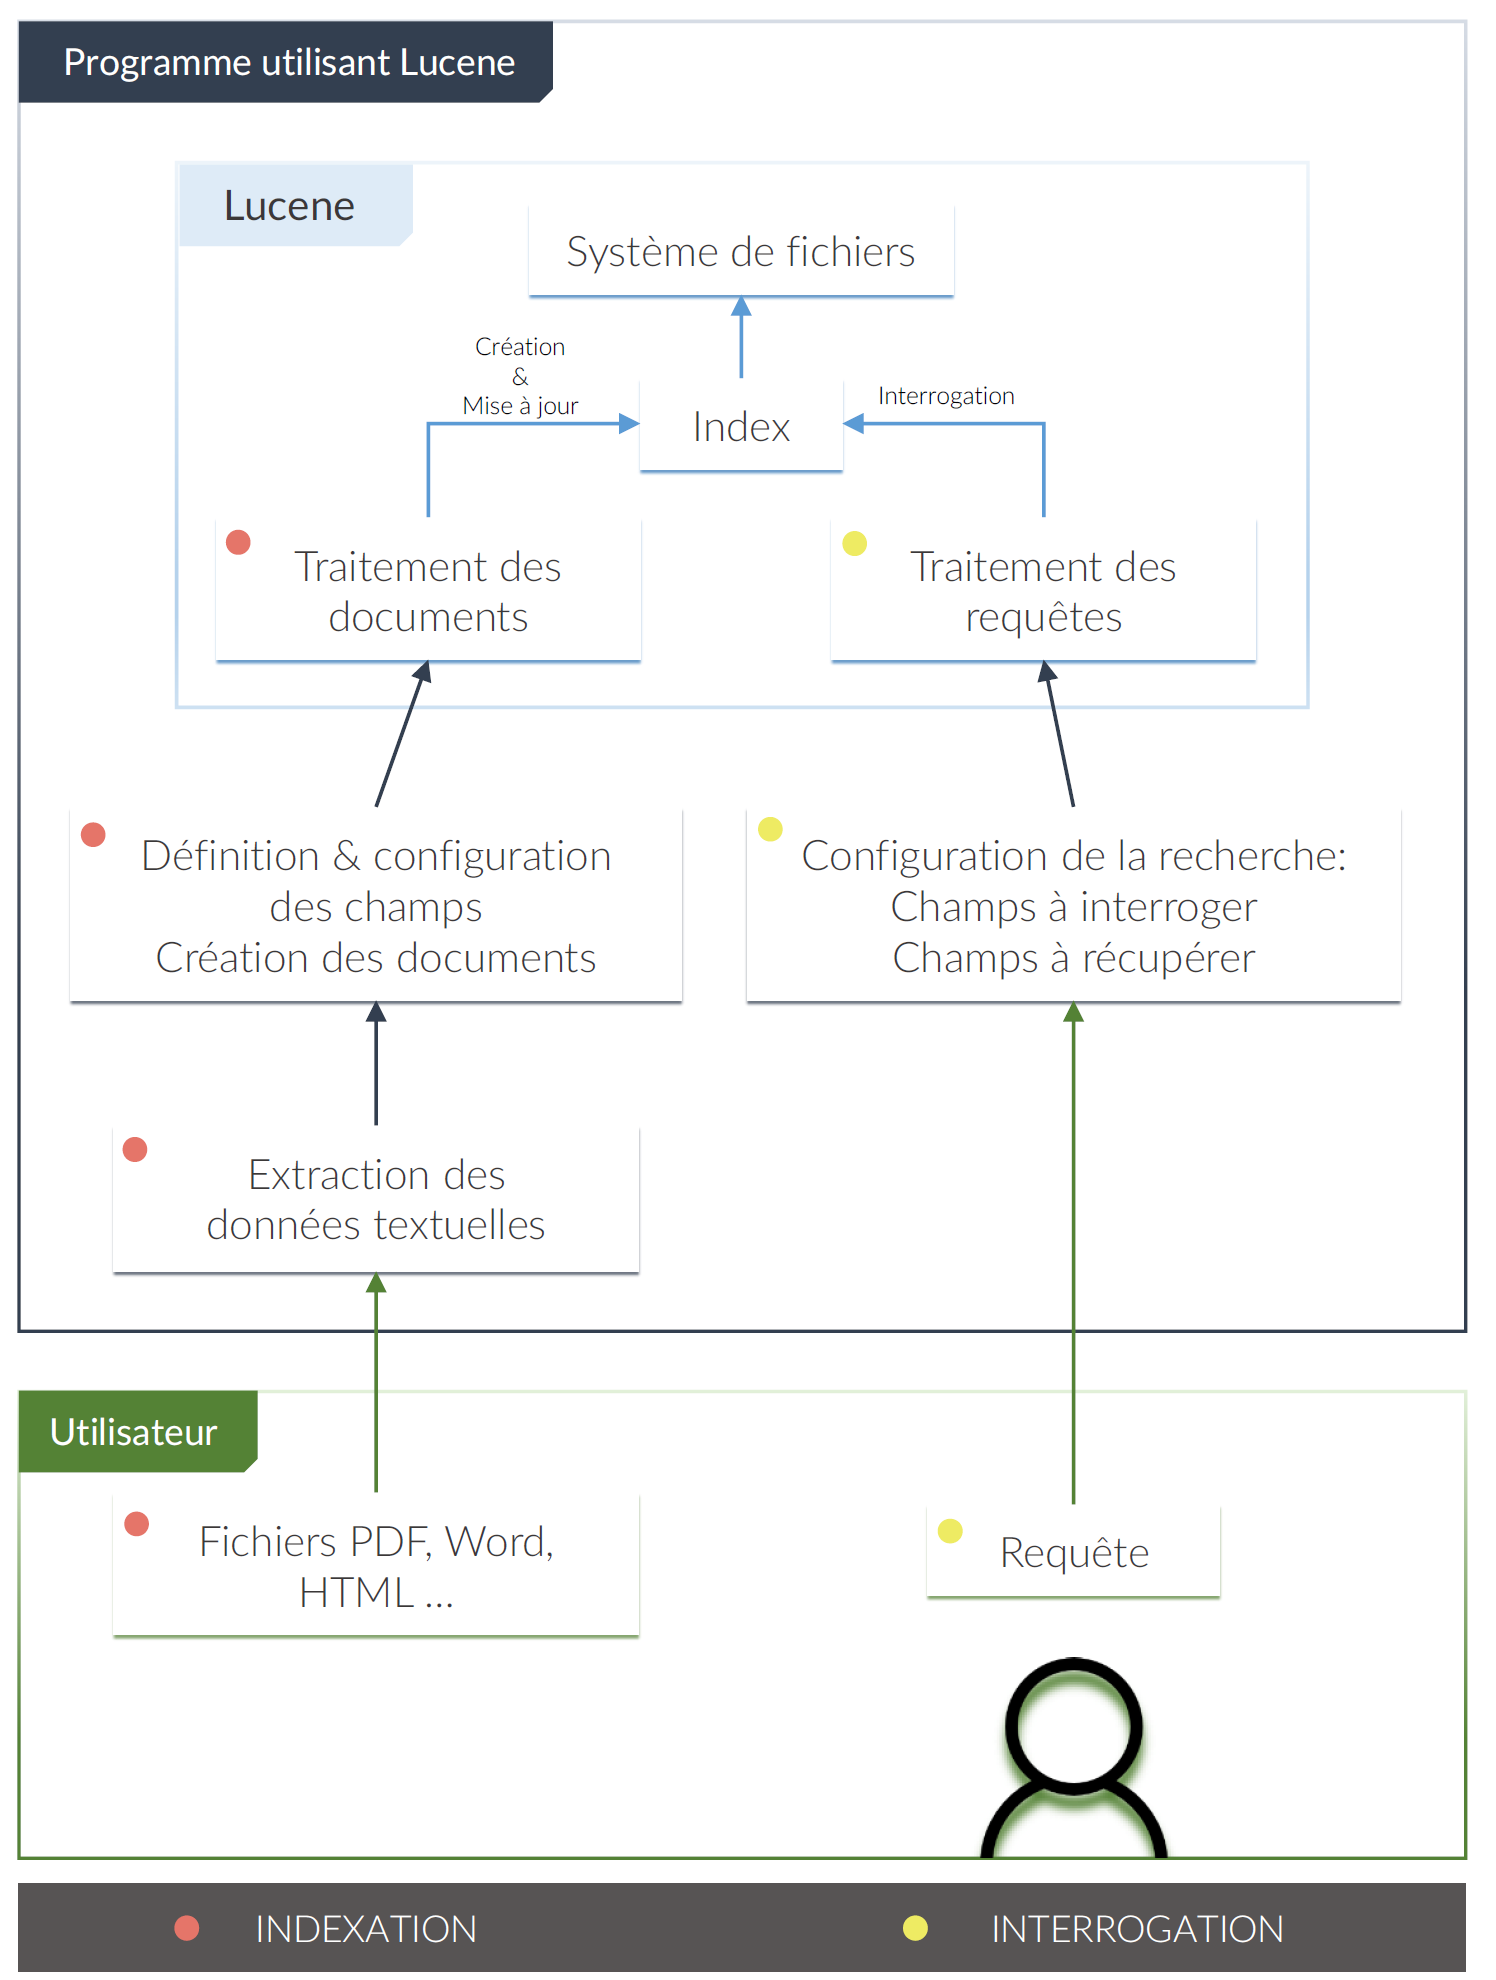
\includegraphics[width=17cm]{figure/fonctionnement.jpg}}
            \end{adjustbox}
      \end{figure}



    % Manoucherie incoming
    %\pagevierge
    %\ifthenelse{\isodd{\thepage}}
    %{\pagevierge}
    %{}
    %
\includepdf[pages=2]{figure/couv.pdf}
\end{document}